% Created by tikzDevice version 0.12.3.1 on 2022-02-03 15:29:14
% !TEX encoding = UTF-8 Unicode
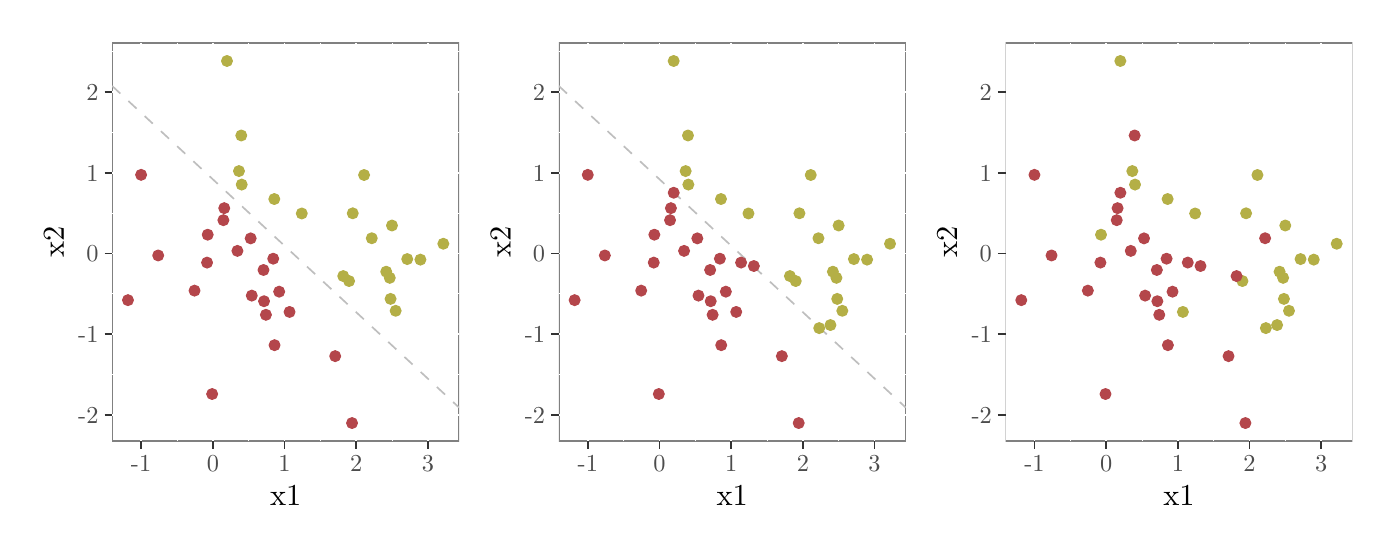
\begin{tikzpicture}[x=1pt,y=1pt]
\definecolor{fillColor}{RGB}{255,255,255}
\path[use as bounding box,fill=fillColor,fill opacity=0.00] (0,0) rectangle (484.21,180.67);
\begin{scope}
\path[clip] (  0.00,  0.00) rectangle (161.40,180.67);
\definecolor{drawColor}{RGB}{255,255,255}
\definecolor{fillColor}{RGB}{255,255,255}

\path[draw=drawColor,line width= 0.6pt,line join=round,line cap=round,fill=fillColor] (  0.00,  0.00) rectangle (161.40,180.68);
\end{scope}
\begin{scope}
\path[clip] ( 30.54, 31.25) rectangle (155.90,175.17);
\definecolor{drawColor}{gray}{0.50}
\definecolor{fillColor}{RGB}{255,255,255}

\path[draw=drawColor,line width= 0.6pt,line join=round,line cap=round,fill=fillColor] ( 30.54, 31.25) rectangle (155.90,175.17);
\definecolor{drawColor}{RGB}{255,255,255}

\path[draw=drawColor,line width= 0.3pt,line join=round] ( 30.54, 55.35) --
	(155.90, 55.35);

\path[draw=drawColor,line width= 0.3pt,line join=round] ( 30.54, 84.49) --
	(155.90, 84.49);

\path[draw=drawColor,line width= 0.3pt,line join=round] ( 30.54,113.63) --
	(155.90,113.63);

\path[draw=drawColor,line width= 0.3pt,line join=round] ( 30.54,142.78) --
	(155.90,142.78);

\path[draw=drawColor,line width= 0.3pt,line join=round] ( 30.54,171.92) --
	(155.90,171.92);

\path[draw=drawColor,line width= 0.3pt,line join=round] ( 53.95, 31.25) --
	( 53.95,175.17);

\path[draw=drawColor,line width= 0.3pt,line join=round] ( 79.86, 31.25) --
	( 79.86,175.17);

\path[draw=drawColor,line width= 0.3pt,line join=round] (105.76, 31.25) --
	(105.76,175.17);

\path[draw=drawColor,line width= 0.3pt,line join=round] (131.67, 31.25) --
	(131.67,175.17);

\path[draw=drawColor,line width= 0.6pt,line join=round] ( 30.54, 40.78) --
	(155.90, 40.78);

\path[draw=drawColor,line width= 0.6pt,line join=round] ( 30.54, 69.92) --
	(155.90, 69.92);

\path[draw=drawColor,line width= 0.6pt,line join=round] ( 30.54, 99.06) --
	(155.90, 99.06);

\path[draw=drawColor,line width= 0.6pt,line join=round] ( 30.54,128.21) --
	(155.90,128.21);

\path[draw=drawColor,line width= 0.6pt,line join=round] ( 30.54,157.35) --
	(155.90,157.35);

\path[draw=drawColor,line width= 0.6pt,line join=round] ( 41.00, 31.25) --
	( 41.00,175.17);

\path[draw=drawColor,line width= 0.6pt,line join=round] ( 66.91, 31.25) --
	( 66.91,175.17);

\path[draw=drawColor,line width= 0.6pt,line join=round] ( 92.81, 31.25) --
	( 92.81,175.17);

\path[draw=drawColor,line width= 0.6pt,line join=round] (118.72, 31.25) --
	(118.72,175.17);

\path[draw=drawColor,line width= 0.6pt,line join=round] (144.62, 31.25) --
	(144.62,175.17);
\definecolor{drawColor}{RGB}{190,190,190}

\path[draw=drawColor,line width= 0.6pt,dash pattern=on 4pt off 4pt ,line join=round] ( 30.54,159.59) -- (155.90, 43.38);
\definecolor{drawColor}{RGB}{180,70,75}
\definecolor{fillColor}{RGB}{180,70,75}

\path[draw=drawColor,line width= 0.4pt,line join=round,line cap=round,fill=fillColor] ( 71.03,115.45) circle (  1.96);

\path[draw=drawColor,line width= 0.4pt,line join=round,line cap=round,fill=fillColor] ( 60.29, 85.65) circle (  1.96);

\path[draw=drawColor,line width= 0.4pt,line join=round,line cap=round,fill=fillColor] ( 94.63, 77.95) circle (  1.96);
\definecolor{drawColor}{RGB}{180,175,70}
\definecolor{fillColor}{RGB}{180,175,70}

\path[draw=drawColor,line width= 0.4pt,line join=round,line cap=round,fill=fillColor] (137.15, 97.05) circle (  1.96);

\path[draw=drawColor,line width= 0.4pt,line join=round,line cap=round,fill=fillColor] ( 77.19,141.71) circle (  1.96);
\definecolor{drawColor}{RGB}{180,70,75}
\definecolor{fillColor}{RGB}{180,70,75}

\path[draw=drawColor,line width= 0.4pt,line join=round,line cap=round,fill=fillColor] ( 80.58,104.53) circle (  1.96);
\definecolor{drawColor}{RGB}{180,175,70}
\definecolor{fillColor}{RGB}{180,175,70}

\path[draw=drawColor,line width= 0.4pt,line join=round,line cap=round,fill=fillColor] ( 76.35,128.85) circle (  1.96);
\definecolor{drawColor}{RGB}{180,70,75}
\definecolor{fillColor}{RGB}{180,70,75}

\path[draw=drawColor,line width= 0.4pt,line join=round,line cap=round,fill=fillColor] ( 85.41, 81.82) circle (  1.96);

\path[draw=drawColor,line width= 0.4pt,line join=round,line cap=round,fill=fillColor] ( 64.82, 95.78) circle (  1.96);

\path[draw=drawColor,line width= 0.4pt,line join=round,line cap=round,fill=fillColor] ( 88.73, 97.19) circle (  1.96);

\path[draw=drawColor,line width= 0.4pt,line join=round,line cap=round,fill=fillColor] ( 65.05,105.86) circle (  1.96);

\path[draw=drawColor,line width= 0.4pt,line join=round,line cap=round,fill=fillColor] ( 89.21, 65.94) circle (  1.96);
\definecolor{drawColor}{RGB}{180,175,70}
\definecolor{fillColor}{RGB}{180,175,70}

\path[draw=drawColor,line width= 0.4pt,line join=round,line cap=round,fill=fillColor] ( 77.34,123.97) circle (  1.96);
\definecolor{drawColor}{RGB}{180,70,75}
\definecolor{fillColor}{RGB}{180,70,75}

\path[draw=drawColor,line width= 0.4pt,line join=round,line cap=round,fill=fillColor] ( 36.24, 82.21) circle (  1.96);
\definecolor{drawColor}{RGB}{180,175,70}
\definecolor{fillColor}{RGB}{180,175,70}

\path[draw=drawColor,line width= 0.4pt,line join=round,line cap=round,fill=fillColor] ( 99.05,113.53) circle (  1.96);
\definecolor{drawColor}{RGB}{180,70,75}
\definecolor{fillColor}{RGB}{180,70,75}

\path[draw=drawColor,line width= 0.4pt,line join=round,line cap=round,fill=fillColor] ( 86.09, 76.91) circle (  1.96);
\definecolor{drawColor}{RGB}{180,175,70}
\definecolor{fillColor}{RGB}{180,175,70}

\path[draw=drawColor,line width= 0.4pt,line join=round,line cap=round,fill=fillColor] (116.14, 89.11) circle (  1.96);
\definecolor{drawColor}{RGB}{180,70,75}
\definecolor{fillColor}{RGB}{180,70,75}

\path[draw=drawColor,line width= 0.4pt,line join=round,line cap=round,fill=fillColor] (117.21, 37.80) circle (  1.96);
\definecolor{drawColor}{RGB}{180,175,70}
\definecolor{fillColor}{RGB}{180,175,70}

\path[draw=drawColor,line width= 0.4pt,line join=round,line cap=round,fill=fillColor] (130.84, 90.27) circle (  1.96);
\definecolor{drawColor}{RGB}{180,70,75}
\definecolor{fillColor}{RGB}{180,70,75}

\path[draw=drawColor,line width= 0.4pt,line join=round,line cap=round,fill=fillColor] (111.12, 61.98) circle (  1.96);
\definecolor{drawColor}{RGB}{180,175,70}
\definecolor{fillColor}{RGB}{180,175,70}

\path[draw=drawColor,line width= 0.4pt,line join=round,line cap=round,fill=fillColor] (114.03, 90.91) circle (  1.96);
\definecolor{drawColor}{RGB}{180,70,75}
\definecolor{fillColor}{RGB}{180,70,75}

\path[draw=drawColor,line width= 0.4pt,line join=round,line cap=round,fill=fillColor] ( 85.21, 93.11) circle (  1.96);
\definecolor{drawColor}{RGB}{180,175,70}
\definecolor{fillColor}{RGB}{180,175,70}

\path[draw=drawColor,line width= 0.4pt,line join=round,line cap=round,fill=fillColor] (129.56, 92.49) circle (  1.96);

\path[draw=drawColor,line width= 0.4pt,line join=round,line cap=round,fill=fillColor] (131.64,109.18) circle (  1.96);
\definecolor{drawColor}{RGB}{180,70,75}
\definecolor{fillColor}{RGB}{180,70,75}

\path[draw=drawColor,line width= 0.4pt,line join=round,line cap=round,fill=fillColor] ( 75.79,100.01) circle (  1.96);

\path[draw=drawColor,line width= 0.4pt,line join=round,line cap=round,fill=fillColor] ( 70.72,111.11) circle (  1.96);
\definecolor{drawColor}{RGB}{180,175,70}
\definecolor{fillColor}{RGB}{180,175,70}

\path[draw=drawColor,line width= 0.4pt,line join=round,line cap=round,fill=fillColor] (121.56,127.43) circle (  1.96);

\path[draw=drawColor,line width= 0.4pt,line join=round,line cap=round,fill=fillColor] (150.20,102.59) circle (  1.96);

\path[draw=drawColor,line width= 0.4pt,line join=round,line cap=round,fill=fillColor] (124.34,104.58) circle (  1.96);

\path[draw=drawColor,line width= 0.4pt,line join=round,line cap=round,fill=fillColor] (131.13, 82.66) circle (  1.96);

\path[draw=drawColor,line width= 0.4pt,line join=round,line cap=round,fill=fillColor] (117.46,113.59) circle (  1.96);
\definecolor{drawColor}{RGB}{180,70,75}
\definecolor{fillColor}{RGB}{180,70,75}

\path[draw=drawColor,line width= 0.4pt,line join=round,line cap=round,fill=fillColor] ( 66.66, 48.29) circle (  1.96);

\path[draw=drawColor,line width= 0.4pt,line join=round,line cap=round,fill=fillColor] ( 40.99,127.49) circle (  1.96);

\path[draw=drawColor,line width= 0.4pt,line join=round,line cap=round,fill=fillColor] ( 47.16, 98.36) circle (  1.96);
\definecolor{drawColor}{RGB}{180,175,70}
\definecolor{fillColor}{RGB}{180,175,70}

\path[draw=drawColor,line width= 0.4pt,line join=round,line cap=round,fill=fillColor] ( 89.12,118.75) circle (  1.96);

\path[draw=drawColor,line width= 0.4pt,line join=round,line cap=round,fill=fillColor] (132.97, 78.36) circle (  1.96);

\path[draw=drawColor,line width= 0.4pt,line join=round,line cap=round,fill=fillColor] ( 72.02,168.63) circle (  1.96);
\definecolor{drawColor}{RGB}{180,70,75}
\definecolor{fillColor}{RGB}{180,70,75}

\path[draw=drawColor,line width= 0.4pt,line join=round,line cap=round,fill=fillColor] ( 90.88, 85.27) circle (  1.96);
\definecolor{drawColor}{RGB}{180,175,70}
\definecolor{fillColor}{RGB}{180,175,70}

\path[draw=drawColor,line width= 0.4pt,line join=round,line cap=round,fill=fillColor] (141.92, 96.85) circle (  1.96);
\definecolor{drawColor}{RGB}{180,70,75}
\definecolor{fillColor}{RGB}{180,70,75}

\path[draw=drawColor,line width= 0.4pt,line join=round,line cap=round,fill=fillColor] ( 80.98, 83.85) circle (  1.96);
\end{scope}
\begin{scope}
\path[clip] (  0.00,  0.00) rectangle (484.21,180.67);
\definecolor{drawColor}{gray}{0.30}

\node[text=drawColor,anchor=base east,inner sep=0pt, outer sep=0pt, scale=  0.88] at ( 25.59, 37.75) {-2};

\node[text=drawColor,anchor=base east,inner sep=0pt, outer sep=0pt, scale=  0.88] at ( 25.59, 66.89) {-1};

\node[text=drawColor,anchor=base east,inner sep=0pt, outer sep=0pt, scale=  0.88] at ( 25.59, 96.03) {0};

\node[text=drawColor,anchor=base east,inner sep=0pt, outer sep=0pt, scale=  0.88] at ( 25.59,125.18) {1};

\node[text=drawColor,anchor=base east,inner sep=0pt, outer sep=0pt, scale=  0.88] at ( 25.59,154.32) {2};
\end{scope}
\begin{scope}
\path[clip] (  0.00,  0.00) rectangle (484.21,180.67);
\definecolor{drawColor}{gray}{0.20}

\path[draw=drawColor,line width= 0.6pt,line join=round] ( 27.79, 40.78) --
	( 30.54, 40.78);

\path[draw=drawColor,line width= 0.6pt,line join=round] ( 27.79, 69.92) --
	( 30.54, 69.92);

\path[draw=drawColor,line width= 0.6pt,line join=round] ( 27.79, 99.06) --
	( 30.54, 99.06);

\path[draw=drawColor,line width= 0.6pt,line join=round] ( 27.79,128.21) --
	( 30.54,128.21);

\path[draw=drawColor,line width= 0.6pt,line join=round] ( 27.79,157.35) --
	( 30.54,157.35);
\end{scope}
\begin{scope}
\path[clip] (  0.00,  0.00) rectangle (484.21,180.67);
\definecolor{drawColor}{gray}{0.20}

\path[draw=drawColor,line width= 0.6pt,line join=round] ( 41.00, 28.50) --
	( 41.00, 31.25);

\path[draw=drawColor,line width= 0.6pt,line join=round] ( 66.91, 28.50) --
	( 66.91, 31.25);

\path[draw=drawColor,line width= 0.6pt,line join=round] ( 92.81, 28.50) --
	( 92.81, 31.25);

\path[draw=drawColor,line width= 0.6pt,line join=round] (118.72, 28.50) --
	(118.72, 31.25);

\path[draw=drawColor,line width= 0.6pt,line join=round] (144.62, 28.50) --
	(144.62, 31.25);
\end{scope}
\begin{scope}
\path[clip] (  0.00,  0.00) rectangle (484.21,180.67);
\definecolor{drawColor}{gray}{0.30}

\node[text=drawColor,anchor=base,inner sep=0pt, outer sep=0pt, scale=  0.88] at ( 41.00, 20.24) {-1};

\node[text=drawColor,anchor=base,inner sep=0pt, outer sep=0pt, scale=  0.88] at ( 66.91, 20.24) {0};

\node[text=drawColor,anchor=base,inner sep=0pt, outer sep=0pt, scale=  0.88] at ( 92.81, 20.24) {1};

\node[text=drawColor,anchor=base,inner sep=0pt, outer sep=0pt, scale=  0.88] at (118.72, 20.24) {2};

\node[text=drawColor,anchor=base,inner sep=0pt, outer sep=0pt, scale=  0.88] at (144.62, 20.24) {3};
\end{scope}
\begin{scope}
\path[clip] (  0.00,  0.00) rectangle (484.21,180.67);
\definecolor{drawColor}{RGB}{0,0,0}

\node[text=drawColor,anchor=base,inner sep=0pt, outer sep=0pt, scale=  1.10] at ( 93.22,  7.93) {x1};
\end{scope}
\begin{scope}
\path[clip] (  0.00,  0.00) rectangle (484.21,180.67);
\definecolor{drawColor}{RGB}{0,0,0}

\node[text=drawColor,rotate= 90.00,anchor=base,inner sep=0pt, outer sep=0pt, scale=  1.10] at ( 13.08,103.21) {x2};
\end{scope}
\begin{scope}
\path[clip] (161.40,  0.00) rectangle (322.81,180.67);
\definecolor{drawColor}{RGB}{255,255,255}
\definecolor{fillColor}{RGB}{255,255,255}

\path[draw=drawColor,line width= 0.6pt,line join=round,line cap=round,fill=fillColor] (161.40,  0.00) rectangle (322.81,180.68);
\end{scope}
\begin{scope}
\path[clip] (191.94, 31.25) rectangle (317.31,175.17);
\definecolor{drawColor}{gray}{0.50}
\definecolor{fillColor}{RGB}{255,255,255}

\path[draw=drawColor,line width= 0.6pt,line join=round,line cap=round,fill=fillColor] (191.94, 31.25) rectangle (317.31,175.17);
\definecolor{drawColor}{RGB}{255,255,255}

\path[draw=drawColor,line width= 0.3pt,line join=round] (191.94, 55.35) --
	(317.31, 55.35);

\path[draw=drawColor,line width= 0.3pt,line join=round] (191.94, 84.49) --
	(317.31, 84.49);

\path[draw=drawColor,line width= 0.3pt,line join=round] (191.94,113.63) --
	(317.31,113.63);

\path[draw=drawColor,line width= 0.3pt,line join=round] (191.94,142.78) --
	(317.31,142.78);

\path[draw=drawColor,line width= 0.3pt,line join=round] (191.94,171.92) --
	(317.31,171.92);

\path[draw=drawColor,line width= 0.3pt,line join=round] (215.36, 31.25) --
	(215.36,175.17);

\path[draw=drawColor,line width= 0.3pt,line join=round] (241.26, 31.25) --
	(241.26,175.17);

\path[draw=drawColor,line width= 0.3pt,line join=round] (267.17, 31.25) --
	(267.17,175.17);

\path[draw=drawColor,line width= 0.3pt,line join=round] (293.07, 31.25) --
	(293.07,175.17);

\path[draw=drawColor,line width= 0.6pt,line join=round] (191.94, 40.78) --
	(317.31, 40.78);

\path[draw=drawColor,line width= 0.6pt,line join=round] (191.94, 69.92) --
	(317.31, 69.92);

\path[draw=drawColor,line width= 0.6pt,line join=round] (191.94, 99.06) --
	(317.31, 99.06);

\path[draw=drawColor,line width= 0.6pt,line join=round] (191.94,128.21) --
	(317.31,128.21);

\path[draw=drawColor,line width= 0.6pt,line join=round] (191.94,157.35) --
	(317.31,157.35);

\path[draw=drawColor,line width= 0.6pt,line join=round] (202.40, 31.25) --
	(202.40,175.17);

\path[draw=drawColor,line width= 0.6pt,line join=round] (228.31, 31.25) --
	(228.31,175.17);

\path[draw=drawColor,line width= 0.6pt,line join=round] (254.21, 31.25) --
	(254.21,175.17);

\path[draw=drawColor,line width= 0.6pt,line join=round] (280.12, 31.25) --
	(280.12,175.17);

\path[draw=drawColor,line width= 0.6pt,line join=round] (306.03, 31.25) --
	(306.03,175.17);
\definecolor{drawColor}{RGB}{190,190,190}

\path[draw=drawColor,line width= 0.6pt,dash pattern=on 4pt off 4pt ,line join=round] (191.94,159.59) -- (317.31, 43.38);
\definecolor{drawColor}{RGB}{180,70,75}
\definecolor{fillColor}{RGB}{180,70,75}

\path[draw=drawColor,line width= 0.4pt,line join=round,line cap=round,fill=fillColor] (232.43,115.45) circle (  1.96);
\definecolor{drawColor}{RGB}{180,175,70}
\definecolor{fillColor}{RGB}{180,175,70}

\path[draw=drawColor,line width= 0.4pt,line join=round,line cap=round,fill=fillColor] (290.08, 73.21) circle (  1.96);
\definecolor{drawColor}{RGB}{180,70,75}
\definecolor{fillColor}{RGB}{180,70,75}

\path[draw=drawColor,line width= 0.4pt,line join=round,line cap=round,fill=fillColor] (221.69, 85.65) circle (  1.96);

\path[draw=drawColor,line width= 0.4pt,line join=round,line cap=round,fill=fillColor] (256.03, 77.95) circle (  1.96);
\definecolor{drawColor}{RGB}{180,175,70}
\definecolor{fillColor}{RGB}{180,175,70}

\path[draw=drawColor,line width= 0.4pt,line join=round,line cap=round,fill=fillColor] (298.55, 97.05) circle (  1.96);

\path[draw=drawColor,line width= 0.4pt,line join=round,line cap=round,fill=fillColor] (238.60,141.71) circle (  1.96);
\definecolor{drawColor}{RGB}{180,70,75}
\definecolor{fillColor}{RGB}{180,70,75}

\path[draw=drawColor,line width= 0.4pt,line join=round,line cap=round,fill=fillColor] (241.98,104.53) circle (  1.96);
\definecolor{drawColor}{RGB}{180,175,70}
\definecolor{fillColor}{RGB}{180,175,70}

\path[draw=drawColor,line width= 0.4pt,line join=round,line cap=round,fill=fillColor] (237.76,128.85) circle (  1.96);
\definecolor{drawColor}{RGB}{180,70,75}
\definecolor{fillColor}{RGB}{180,70,75}

\path[draw=drawColor,line width= 0.4pt,line join=round,line cap=round,fill=fillColor] (246.81, 81.82) circle (  1.96);

\path[draw=drawColor,line width= 0.4pt,line join=round,line cap=round,fill=fillColor] (257.79, 95.79) circle (  1.96);
\definecolor{drawColor}{RGB}{180,175,70}
\definecolor{fillColor}{RGB}{180,175,70}

\path[draw=drawColor,line width= 0.4pt,line join=round,line cap=round,fill=fillColor] (286.02, 72.11) circle (  1.96);
\definecolor{drawColor}{RGB}{180,70,75}
\definecolor{fillColor}{RGB}{180,70,75}

\path[draw=drawColor,line width= 0.4pt,line join=round,line cap=round,fill=fillColor] (233.44,121.02) circle (  1.96);

\path[draw=drawColor,line width= 0.4pt,line join=round,line cap=round,fill=fillColor] (226.23, 95.78) circle (  1.96);

\path[draw=drawColor,line width= 0.4pt,line join=round,line cap=round,fill=fillColor] (250.13, 97.19) circle (  1.96);

\path[draw=drawColor,line width= 0.4pt,line join=round,line cap=round,fill=fillColor] (226.45,105.86) circle (  1.96);

\path[draw=drawColor,line width= 0.4pt,line join=round,line cap=round,fill=fillColor] (250.61, 65.94) circle (  1.96);
\definecolor{drawColor}{RGB}{180,175,70}
\definecolor{fillColor}{RGB}{180,175,70}

\path[draw=drawColor,line width= 0.4pt,line join=round,line cap=round,fill=fillColor] (238.74,123.97) circle (  1.96);
\definecolor{drawColor}{RGB}{180,70,75}
\definecolor{fillColor}{RGB}{180,70,75}

\path[draw=drawColor,line width= 0.4pt,line join=round,line cap=round,fill=fillColor] (197.64, 82.21) circle (  1.96);
\definecolor{drawColor}{RGB}{180,175,70}
\definecolor{fillColor}{RGB}{180,175,70}

\path[draw=drawColor,line width= 0.4pt,line join=round,line cap=round,fill=fillColor] (260.45,113.53) circle (  1.96);
\definecolor{drawColor}{RGB}{180,70,75}
\definecolor{fillColor}{RGB}{180,70,75}

\path[draw=drawColor,line width= 0.4pt,line join=round,line cap=round,fill=fillColor] (247.50, 76.91) circle (  1.96);
\definecolor{drawColor}{RGB}{180,175,70}
\definecolor{fillColor}{RGB}{180,175,70}

\path[draw=drawColor,line width= 0.4pt,line join=round,line cap=round,fill=fillColor] (277.54, 89.11) circle (  1.96);
\definecolor{drawColor}{RGB}{180,70,75}
\definecolor{fillColor}{RGB}{180,70,75}

\path[draw=drawColor,line width= 0.4pt,line join=round,line cap=round,fill=fillColor] (278.61, 37.80) circle (  1.96);
\definecolor{drawColor}{RGB}{180,175,70}
\definecolor{fillColor}{RGB}{180,175,70}

\path[draw=drawColor,line width= 0.4pt,line join=round,line cap=round,fill=fillColor] (292.24, 90.27) circle (  1.96);
\definecolor{drawColor}{RGB}{180,70,75}
\definecolor{fillColor}{RGB}{180,70,75}

\path[draw=drawColor,line width= 0.4pt,line join=round,line cap=round,fill=fillColor] (272.52, 61.98) circle (  1.96);
\definecolor{drawColor}{RGB}{180,175,70}
\definecolor{fillColor}{RGB}{180,175,70}

\path[draw=drawColor,line width= 0.4pt,line join=round,line cap=round,fill=fillColor] (275.43, 90.91) circle (  1.96);
\definecolor{drawColor}{RGB}{180,70,75}
\definecolor{fillColor}{RGB}{180,70,75}

\path[draw=drawColor,line width= 0.4pt,line join=round,line cap=round,fill=fillColor] (246.61, 93.11) circle (  1.96);
\definecolor{drawColor}{RGB}{180,175,70}
\definecolor{fillColor}{RGB}{180,175,70}

\path[draw=drawColor,line width= 0.4pt,line join=round,line cap=round,fill=fillColor] (290.96, 92.49) circle (  1.96);

\path[draw=drawColor,line width= 0.4pt,line join=round,line cap=round,fill=fillColor] (293.04,109.18) circle (  1.96);
\definecolor{drawColor}{RGB}{180,70,75}
\definecolor{fillColor}{RGB}{180,70,75}

\path[draw=drawColor,line width= 0.4pt,line join=round,line cap=round,fill=fillColor] (237.19,100.01) circle (  1.96);

\path[draw=drawColor,line width= 0.4pt,line join=round,line cap=round,fill=fillColor] (232.12,111.11) circle (  1.96);

\path[draw=drawColor,line width= 0.4pt,line join=round,line cap=round,fill=fillColor] (262.40, 94.54) circle (  1.96);
\definecolor{drawColor}{RGB}{180,175,70}
\definecolor{fillColor}{RGB}{180,175,70}

\path[draw=drawColor,line width= 0.4pt,line join=round,line cap=round,fill=fillColor] (282.96,127.43) circle (  1.96);

\path[draw=drawColor,line width= 0.4pt,line join=round,line cap=round,fill=fillColor] (311.61,102.59) circle (  1.96);

\path[draw=drawColor,line width= 0.4pt,line join=round,line cap=round,fill=fillColor] (285.74,104.58) circle (  1.96);

\path[draw=drawColor,line width= 0.4pt,line join=round,line cap=round,fill=fillColor] (292.53, 82.66) circle (  1.96);

\path[draw=drawColor,line width= 0.4pt,line join=round,line cap=round,fill=fillColor] (278.87,113.59) circle (  1.96);
\definecolor{drawColor}{RGB}{180,70,75}
\definecolor{fillColor}{RGB}{180,70,75}

\path[draw=drawColor,line width= 0.4pt,line join=round,line cap=round,fill=fillColor] (228.06, 48.29) circle (  1.96);

\path[draw=drawColor,line width= 0.4pt,line join=round,line cap=round,fill=fillColor] (202.39,127.49) circle (  1.96);

\path[draw=drawColor,line width= 0.4pt,line join=round,line cap=round,fill=fillColor] (208.56, 98.36) circle (  1.96);
\definecolor{drawColor}{RGB}{180,175,70}
\definecolor{fillColor}{RGB}{180,175,70}

\path[draw=drawColor,line width= 0.4pt,line join=round,line cap=round,fill=fillColor] (250.52,118.75) circle (  1.96);

\path[draw=drawColor,line width= 0.4pt,line join=round,line cap=round,fill=fillColor] (294.37, 78.36) circle (  1.96);

\path[draw=drawColor,line width= 0.4pt,line join=round,line cap=round,fill=fillColor] (233.43,168.63) circle (  1.96);
\definecolor{drawColor}{RGB}{180,70,75}
\definecolor{fillColor}{RGB}{180,70,75}

\path[draw=drawColor,line width= 0.4pt,line join=round,line cap=round,fill=fillColor] (252.28, 85.27) circle (  1.96);
\definecolor{drawColor}{RGB}{180,175,70}
\definecolor{fillColor}{RGB}{180,175,70}

\path[draw=drawColor,line width= 0.4pt,line join=round,line cap=round,fill=fillColor] (303.32, 96.85) circle (  1.96);
\definecolor{drawColor}{RGB}{180,70,75}
\definecolor{fillColor}{RGB}{180,70,75}

\path[draw=drawColor,line width= 0.4pt,line join=round,line cap=round,fill=fillColor] (242.39, 83.85) circle (  1.96);
\end{scope}
\begin{scope}
\path[clip] (  0.00,  0.00) rectangle (484.21,180.67);
\definecolor{drawColor}{gray}{0.30}

\node[text=drawColor,anchor=base east,inner sep=0pt, outer sep=0pt, scale=  0.88] at (186.99, 37.75) {-2};

\node[text=drawColor,anchor=base east,inner sep=0pt, outer sep=0pt, scale=  0.88] at (186.99, 66.89) {-1};

\node[text=drawColor,anchor=base east,inner sep=0pt, outer sep=0pt, scale=  0.88] at (186.99, 96.03) {0};

\node[text=drawColor,anchor=base east,inner sep=0pt, outer sep=0pt, scale=  0.88] at (186.99,125.18) {1};

\node[text=drawColor,anchor=base east,inner sep=0pt, outer sep=0pt, scale=  0.88] at (186.99,154.32) {2};
\end{scope}
\begin{scope}
\path[clip] (  0.00,  0.00) rectangle (484.21,180.67);
\definecolor{drawColor}{gray}{0.20}

\path[draw=drawColor,line width= 0.6pt,line join=round] (189.19, 40.78) --
	(191.94, 40.78);

\path[draw=drawColor,line width= 0.6pt,line join=round] (189.19, 69.92) --
	(191.94, 69.92);

\path[draw=drawColor,line width= 0.6pt,line join=round] (189.19, 99.06) --
	(191.94, 99.06);

\path[draw=drawColor,line width= 0.6pt,line join=round] (189.19,128.21) --
	(191.94,128.21);

\path[draw=drawColor,line width= 0.6pt,line join=round] (189.19,157.35) --
	(191.94,157.35);
\end{scope}
\begin{scope}
\path[clip] (  0.00,  0.00) rectangle (484.21,180.67);
\definecolor{drawColor}{gray}{0.20}

\path[draw=drawColor,line width= 0.6pt,line join=round] (202.40, 28.50) --
	(202.40, 31.25);

\path[draw=drawColor,line width= 0.6pt,line join=round] (228.31, 28.50) --
	(228.31, 31.25);

\path[draw=drawColor,line width= 0.6pt,line join=round] (254.21, 28.50) --
	(254.21, 31.25);

\path[draw=drawColor,line width= 0.6pt,line join=round] (280.12, 28.50) --
	(280.12, 31.25);

\path[draw=drawColor,line width= 0.6pt,line join=round] (306.03, 28.50) --
	(306.03, 31.25);
\end{scope}
\begin{scope}
\path[clip] (  0.00,  0.00) rectangle (484.21,180.67);
\definecolor{drawColor}{gray}{0.30}

\node[text=drawColor,anchor=base,inner sep=0pt, outer sep=0pt, scale=  0.88] at (202.40, 20.24) {-1};

\node[text=drawColor,anchor=base,inner sep=0pt, outer sep=0pt, scale=  0.88] at (228.31, 20.24) {0};

\node[text=drawColor,anchor=base,inner sep=0pt, outer sep=0pt, scale=  0.88] at (254.21, 20.24) {1};

\node[text=drawColor,anchor=base,inner sep=0pt, outer sep=0pt, scale=  0.88] at (280.12, 20.24) {2};

\node[text=drawColor,anchor=base,inner sep=0pt, outer sep=0pt, scale=  0.88] at (306.03, 20.24) {3};
\end{scope}
\begin{scope}
\path[clip] (  0.00,  0.00) rectangle (484.21,180.67);
\definecolor{drawColor}{RGB}{0,0,0}

\node[text=drawColor,anchor=base,inner sep=0pt, outer sep=0pt, scale=  1.10] at (254.62,  7.93) {x1};
\end{scope}
\begin{scope}
\path[clip] (  0.00,  0.00) rectangle (484.21,180.67);
\definecolor{drawColor}{RGB}{0,0,0}

\node[text=drawColor,rotate= 90.00,anchor=base,inner sep=0pt, outer sep=0pt, scale=  1.10] at (174.48,103.21) {x2};
\end{scope}
\begin{scope}
\path[clip] (322.81,  0.00) rectangle (484.21,180.67);
\definecolor{drawColor}{RGB}{255,255,255}
\definecolor{fillColor}{RGB}{255,255,255}

\path[draw=drawColor,line width= 0.6pt,line join=round,line cap=round,fill=fillColor] (322.81,  0.00) rectangle (484.21,180.68);
\end{scope}
\begin{scope}
\path[clip] (353.34, 31.25) rectangle (478.71,175.17);
\definecolor{drawColor}{gray}{0.50}
\definecolor{fillColor}{RGB}{255,255,255}

\path[draw=drawColor,line width= 0.6pt,line join=round,line cap=round,fill=fillColor] (353.34, 31.25) rectangle (478.71,175.17);
\definecolor{drawColor}{RGB}{255,255,255}

\path[draw=drawColor,line width= 0.3pt,line join=round] (353.34, 55.35) --
	(478.71, 55.35);

\path[draw=drawColor,line width= 0.3pt,line join=round] (353.34, 84.49) --
	(478.71, 84.49);

\path[draw=drawColor,line width= 0.3pt,line join=round] (353.34,113.63) --
	(478.71,113.63);

\path[draw=drawColor,line width= 0.3pt,line join=round] (353.34,142.78) --
	(478.71,142.78);

\path[draw=drawColor,line width= 0.3pt,line join=round] (353.34,171.92) --
	(478.71,171.92);

\path[draw=drawColor,line width= 0.3pt,line join=round] (376.76, 31.25) --
	(376.76,175.17);

\path[draw=drawColor,line width= 0.3pt,line join=round] (402.67, 31.25) --
	(402.67,175.17);

\path[draw=drawColor,line width= 0.3pt,line join=round] (428.57, 31.25) --
	(428.57,175.17);

\path[draw=drawColor,line width= 0.3pt,line join=round] (454.48, 31.25) --
	(454.48,175.17);

\path[draw=drawColor,line width= 0.6pt,line join=round] (353.34, 40.78) --
	(478.71, 40.78);

\path[draw=drawColor,line width= 0.6pt,line join=round] (353.34, 69.92) --
	(478.71, 69.92);

\path[draw=drawColor,line width= 0.6pt,line join=round] (353.34, 99.06) --
	(478.71, 99.06);

\path[draw=drawColor,line width= 0.6pt,line join=round] (353.34,128.21) --
	(478.71,128.21);

\path[draw=drawColor,line width= 0.6pt,line join=round] (353.34,157.35) --
	(478.71,157.35);

\path[draw=drawColor,line width= 0.6pt,line join=round] (363.81, 31.25) --
	(363.81,175.17);

\path[draw=drawColor,line width= 0.6pt,line join=round] (389.71, 31.25) --
	(389.71,175.17);

\path[draw=drawColor,line width= 0.6pt,line join=round] (415.62, 31.25) --
	(415.62,175.17);

\path[draw=drawColor,line width= 0.6pt,line join=round] (441.52, 31.25) --
	(441.52,175.17);

\path[draw=drawColor,line width= 0.6pt,line join=round] (467.43, 31.25) --
	(467.43,175.17);
\definecolor{drawColor}{RGB}{180,70,75}
\definecolor{fillColor}{RGB}{180,70,75}

\path[draw=drawColor,line width= 0.4pt,line join=round,line cap=round,fill=fillColor] (393.84,115.45) circle (  1.96);
\definecolor{drawColor}{RGB}{180,175,70}
\definecolor{fillColor}{RGB}{180,175,70}

\path[draw=drawColor,line width= 0.4pt,line join=round,line cap=round,fill=fillColor] (451.48, 73.21) circle (  1.96);
\definecolor{drawColor}{RGB}{180,70,75}
\definecolor{fillColor}{RGB}{180,70,75}

\path[draw=drawColor,line width= 0.4pt,line join=round,line cap=round,fill=fillColor] (383.09, 85.65) circle (  1.96);
\definecolor{drawColor}{RGB}{180,175,70}
\definecolor{fillColor}{RGB}{180,175,70}

\path[draw=drawColor,line width= 0.4pt,line join=round,line cap=round,fill=fillColor] (417.43, 77.95) circle (  1.96);

\path[draw=drawColor,line width= 0.4pt,line join=round,line cap=round,fill=fillColor] (459.95, 97.05) circle (  1.96);
\definecolor{drawColor}{RGB}{180,70,75}
\definecolor{fillColor}{RGB}{180,70,75}

\path[draw=drawColor,line width= 0.4pt,line join=round,line cap=round,fill=fillColor] (400.00,141.71) circle (  1.96);

\path[draw=drawColor,line width= 0.4pt,line join=round,line cap=round,fill=fillColor] (403.39,104.53) circle (  1.96);
\definecolor{drawColor}{RGB}{180,175,70}
\definecolor{fillColor}{RGB}{180,175,70}

\path[draw=drawColor,line width= 0.4pt,line join=round,line cap=round,fill=fillColor] (399.16,128.85) circle (  1.96);
\definecolor{drawColor}{RGB}{180,70,75}
\definecolor{fillColor}{RGB}{180,70,75}

\path[draw=drawColor,line width= 0.4pt,line join=round,line cap=round,fill=fillColor] (408.21, 81.82) circle (  1.96);

\path[draw=drawColor,line width= 0.4pt,line join=round,line cap=round,fill=fillColor] (419.20, 95.79) circle (  1.96);
\definecolor{drawColor}{RGB}{180,175,70}
\definecolor{fillColor}{RGB}{180,175,70}

\path[draw=drawColor,line width= 0.4pt,line join=round,line cap=round,fill=fillColor] (447.42, 72.11) circle (  1.96);
\definecolor{drawColor}{RGB}{180,70,75}
\definecolor{fillColor}{RGB}{180,70,75}

\path[draw=drawColor,line width= 0.4pt,line join=round,line cap=round,fill=fillColor] (394.85,121.02) circle (  1.96);

\path[draw=drawColor,line width= 0.4pt,line join=round,line cap=round,fill=fillColor] (387.63, 95.78) circle (  1.96);

\path[draw=drawColor,line width= 0.4pt,line join=round,line cap=round,fill=fillColor] (411.54, 97.19) circle (  1.96);
\definecolor{drawColor}{RGB}{180,175,70}
\definecolor{fillColor}{RGB}{180,175,70}

\path[draw=drawColor,line width= 0.4pt,line join=round,line cap=round,fill=fillColor] (387.85,105.86) circle (  1.96);
\definecolor{drawColor}{RGB}{180,70,75}
\definecolor{fillColor}{RGB}{180,70,75}

\path[draw=drawColor,line width= 0.4pt,line join=round,line cap=round,fill=fillColor] (412.02, 65.94) circle (  1.96);
\definecolor{drawColor}{RGB}{180,175,70}
\definecolor{fillColor}{RGB}{180,175,70}

\path[draw=drawColor,line width= 0.4pt,line join=round,line cap=round,fill=fillColor] (400.14,123.97) circle (  1.96);
\definecolor{drawColor}{RGB}{180,70,75}
\definecolor{fillColor}{RGB}{180,70,75}

\path[draw=drawColor,line width= 0.4pt,line join=round,line cap=round,fill=fillColor] (359.04, 82.21) circle (  1.96);
\definecolor{drawColor}{RGB}{180,175,70}
\definecolor{fillColor}{RGB}{180,175,70}

\path[draw=drawColor,line width= 0.4pt,line join=round,line cap=round,fill=fillColor] (421.86,113.53) circle (  1.96);
\definecolor{drawColor}{RGB}{180,70,75}
\definecolor{fillColor}{RGB}{180,70,75}

\path[draw=drawColor,line width= 0.4pt,line join=round,line cap=round,fill=fillColor] (408.90, 76.91) circle (  1.96);
\definecolor{drawColor}{RGB}{180,175,70}
\definecolor{fillColor}{RGB}{180,175,70}

\path[draw=drawColor,line width= 0.4pt,line join=round,line cap=round,fill=fillColor] (438.95, 89.11) circle (  1.96);
\definecolor{drawColor}{RGB}{180,70,75}
\definecolor{fillColor}{RGB}{180,70,75}

\path[draw=drawColor,line width= 0.4pt,line join=round,line cap=round,fill=fillColor] (440.02, 37.80) circle (  1.96);
\definecolor{drawColor}{RGB}{180,175,70}
\definecolor{fillColor}{RGB}{180,175,70}

\path[draw=drawColor,line width= 0.4pt,line join=round,line cap=round,fill=fillColor] (453.65, 90.27) circle (  1.96);
\definecolor{drawColor}{RGB}{180,70,75}
\definecolor{fillColor}{RGB}{180,70,75}

\path[draw=drawColor,line width= 0.4pt,line join=round,line cap=round,fill=fillColor] (433.93, 61.98) circle (  1.96);

\path[draw=drawColor,line width= 0.4pt,line join=round,line cap=round,fill=fillColor] (436.83, 90.91) circle (  1.96);

\path[draw=drawColor,line width= 0.4pt,line join=round,line cap=round,fill=fillColor] (408.02, 93.11) circle (  1.96);
\definecolor{drawColor}{RGB}{180,175,70}
\definecolor{fillColor}{RGB}{180,175,70}

\path[draw=drawColor,line width= 0.4pt,line join=round,line cap=round,fill=fillColor] (452.37, 92.49) circle (  1.96);

\path[draw=drawColor,line width= 0.4pt,line join=round,line cap=round,fill=fillColor] (454.44,109.18) circle (  1.96);
\definecolor{drawColor}{RGB}{180,70,75}
\definecolor{fillColor}{RGB}{180,70,75}

\path[draw=drawColor,line width= 0.4pt,line join=round,line cap=round,fill=fillColor] (398.60,100.01) circle (  1.96);

\path[draw=drawColor,line width= 0.4pt,line join=round,line cap=round,fill=fillColor] (393.53,111.11) circle (  1.96);

\path[draw=drawColor,line width= 0.4pt,line join=round,line cap=round,fill=fillColor] (423.80, 94.54) circle (  1.96);
\definecolor{drawColor}{RGB}{180,175,70}
\definecolor{fillColor}{RGB}{180,175,70}

\path[draw=drawColor,line width= 0.4pt,line join=round,line cap=round,fill=fillColor] (444.37,127.43) circle (  1.96);

\path[draw=drawColor,line width= 0.4pt,line join=round,line cap=round,fill=fillColor] (473.01,102.59) circle (  1.96);
\definecolor{drawColor}{RGB}{180,70,75}
\definecolor{fillColor}{RGB}{180,70,75}

\path[draw=drawColor,line width= 0.4pt,line join=round,line cap=round,fill=fillColor] (447.15,104.58) circle (  1.96);
\definecolor{drawColor}{RGB}{180,175,70}
\definecolor{fillColor}{RGB}{180,175,70}

\path[draw=drawColor,line width= 0.4pt,line join=round,line cap=round,fill=fillColor] (453.94, 82.66) circle (  1.96);

\path[draw=drawColor,line width= 0.4pt,line join=round,line cap=round,fill=fillColor] (440.27,113.59) circle (  1.96);
\definecolor{drawColor}{RGB}{180,70,75}
\definecolor{fillColor}{RGB}{180,70,75}

\path[draw=drawColor,line width= 0.4pt,line join=round,line cap=round,fill=fillColor] (389.47, 48.29) circle (  1.96);

\path[draw=drawColor,line width= 0.4pt,line join=round,line cap=round,fill=fillColor] (363.79,127.49) circle (  1.96);

\path[draw=drawColor,line width= 0.4pt,line join=round,line cap=round,fill=fillColor] (369.97, 98.36) circle (  1.96);
\definecolor{drawColor}{RGB}{180,175,70}
\definecolor{fillColor}{RGB}{180,175,70}

\path[draw=drawColor,line width= 0.4pt,line join=round,line cap=round,fill=fillColor] (411.92,118.75) circle (  1.96);

\path[draw=drawColor,line width= 0.4pt,line join=round,line cap=round,fill=fillColor] (455.77, 78.36) circle (  1.96);

\path[draw=drawColor,line width= 0.4pt,line join=round,line cap=round,fill=fillColor] (394.83,168.63) circle (  1.96);
\definecolor{drawColor}{RGB}{180,70,75}
\definecolor{fillColor}{RGB}{180,70,75}

\path[draw=drawColor,line width= 0.4pt,line join=round,line cap=round,fill=fillColor] (413.69, 85.27) circle (  1.96);
\definecolor{drawColor}{RGB}{180,175,70}
\definecolor{fillColor}{RGB}{180,175,70}

\path[draw=drawColor,line width= 0.4pt,line join=round,line cap=round,fill=fillColor] (464.73, 96.85) circle (  1.96);
\definecolor{drawColor}{RGB}{180,70,75}
\definecolor{fillColor}{RGB}{180,70,75}

\path[draw=drawColor,line width= 0.4pt,line join=round,line cap=round,fill=fillColor] (403.79, 83.85) circle (  1.96);
\end{scope}
\begin{scope}
\path[clip] (  0.00,  0.00) rectangle (484.21,180.67);
\definecolor{drawColor}{gray}{0.30}

\node[text=drawColor,anchor=base east,inner sep=0pt, outer sep=0pt, scale=  0.88] at (348.39, 37.75) {-2};

\node[text=drawColor,anchor=base east,inner sep=0pt, outer sep=0pt, scale=  0.88] at (348.39, 66.89) {-1};

\node[text=drawColor,anchor=base east,inner sep=0pt, outer sep=0pt, scale=  0.88] at (348.39, 96.03) {0};

\node[text=drawColor,anchor=base east,inner sep=0pt, outer sep=0pt, scale=  0.88] at (348.39,125.18) {1};

\node[text=drawColor,anchor=base east,inner sep=0pt, outer sep=0pt, scale=  0.88] at (348.39,154.32) {2};
\end{scope}
\begin{scope}
\path[clip] (  0.00,  0.00) rectangle (484.21,180.67);
\definecolor{drawColor}{gray}{0.20}

\path[draw=drawColor,line width= 0.6pt,line join=round] (350.59, 40.78) --
	(353.34, 40.78);

\path[draw=drawColor,line width= 0.6pt,line join=round] (350.59, 69.92) --
	(353.34, 69.92);

\path[draw=drawColor,line width= 0.6pt,line join=round] (350.59, 99.06) --
	(353.34, 99.06);

\path[draw=drawColor,line width= 0.6pt,line join=round] (350.59,128.21) --
	(353.34,128.21);

\path[draw=drawColor,line width= 0.6pt,line join=round] (350.59,157.35) --
	(353.34,157.35);
\end{scope}
\begin{scope}
\path[clip] (  0.00,  0.00) rectangle (484.21,180.67);
\definecolor{drawColor}{gray}{0.20}

\path[draw=drawColor,line width= 0.6pt,line join=round] (363.81, 28.50) --
	(363.81, 31.25);

\path[draw=drawColor,line width= 0.6pt,line join=round] (389.71, 28.50) --
	(389.71, 31.25);

\path[draw=drawColor,line width= 0.6pt,line join=round] (415.62, 28.50) --
	(415.62, 31.25);

\path[draw=drawColor,line width= 0.6pt,line join=round] (441.52, 28.50) --
	(441.52, 31.25);

\path[draw=drawColor,line width= 0.6pt,line join=round] (467.43, 28.50) --
	(467.43, 31.25);
\end{scope}
\begin{scope}
\path[clip] (  0.00,  0.00) rectangle (484.21,180.67);
\definecolor{drawColor}{gray}{0.30}

\node[text=drawColor,anchor=base,inner sep=0pt, outer sep=0pt, scale=  0.88] at (363.81, 20.24) {-1};

\node[text=drawColor,anchor=base,inner sep=0pt, outer sep=0pt, scale=  0.88] at (389.71, 20.24) {0};

\node[text=drawColor,anchor=base,inner sep=0pt, outer sep=0pt, scale=  0.88] at (415.62, 20.24) {1};

\node[text=drawColor,anchor=base,inner sep=0pt, outer sep=0pt, scale=  0.88] at (441.52, 20.24) {2};

\node[text=drawColor,anchor=base,inner sep=0pt, outer sep=0pt, scale=  0.88] at (467.43, 20.24) {3};
\end{scope}
\begin{scope}
\path[clip] (  0.00,  0.00) rectangle (484.21,180.67);
\definecolor{drawColor}{RGB}{0,0,0}

\node[text=drawColor,anchor=base,inner sep=0pt, outer sep=0pt, scale=  1.10] at (416.03,  7.93) {x1};
\end{scope}
\begin{scope}
\path[clip] (  0.00,  0.00) rectangle (484.21,180.67);
\definecolor{drawColor}{RGB}{0,0,0}

\node[text=drawColor,rotate= 90.00,anchor=base,inner sep=0pt, outer sep=0pt, scale=  1.10] at (335.88,103.21) {x2};
\end{scope}
\end{tikzpicture}
